\documentclass[11pt,a4paper]{article}

\usepackage[margin=1in]{geometry}
\usepackage{titlesec}
\usepackage{enumitem}
\usepackage{hyperref}
\usepackage{parskip}
\usepackage{graphicx}
\usepackage{float}
\usepackage{booktabs}
\usepackage{amsmath}
\usepackage{amssymb}

\hypersetup{colorlinks=true, linkcolor=blue, urlcolor=blue}

\titleformat{\section}{\large\bfseries}{\thesection}{0.5em}{}
\titleformat{\subsection}{\normalsize\bfseries}{\thesubsection}{0.5em}{}
\setlist{leftmargin=1.4em, topsep=2pt, itemsep=2pt}

\title{\vspace{-1.5cm}\textbf{PKCERT AI \& Software Development Internship \\ Task 27: NLP Basics -- Tokenization, Word Embeddings, and Hugging Face Transformers}}
\author{Abdullah Amir}
\date{AI and Software Development \\ 17 August 2026}

\begin{document}

\maketitle
\vspace{-0.8cm}

Full code lives in \texttt{Day\_27.ipynb} and the standalone scripts it is built from.
\textbf{Pure Python, no external tokenizer library}, for Part A's from-scratch BPE
implementation, per the brief's explicit restriction for that sub-task -- \textbf{gensim}
(Word2Vec), pretrained \textbf{GloVe} vectors, and \textbf{Hugging Face
\texttt{transformers}} (DistilBERT) for Parts B/C, none reimplemented from scratch. Random
seed \textbf{42} throughout.

% ----------------------------------------------------------------
\section*{Part A: Tokenization Foundations}

\textbf{A1 -- word/character/subword trade-offs.} \textbf{Word-level}: short sequences,
semantically meaningful tokens; unbounded vocabulary and total-information-loss OOV handling
(every unseen word collapses to one \texttt{<unk>}). \textbf{Character-level}: tiny, fixed
vocabulary, near-zero true OOV; long sequences, low per-token semantic content, harder
credit assignment. \textbf{Subword-level}: the practical middle ground -- frequent whole
words stay single tokens, rare/unseen words decompose into frequent pieces, bounding
vocabulary while keeping OOV words \emph{meaningfully} represented rather than discarded.

\textbf{A2 -- BPE, derived.} Represent each corpus word as characters + an end-of-word marker
\texttt{</w>} (prevents merges spanning word boundaries); initialize the vocabulary as all
individual characters; repeatedly count every adjacent symbol-pair's frequency (weighted by
word frequency), merge the single most frequent pair everywhere it occurs, and record the
merge. Encoding a new word applies the learned merges, in order, to its character sequence --
any substring matching no merge stays as individual characters, so BPE always produces
\emph{something} meaningful for a novel word, never a single \texttt{<unk>}.

\textbf{A4 -- from-scratch implementation.} \texttt{SimpleBPE}, trained on a 6-sentence
corpus, 40-merge budget:

\begin{table}[H]
\centering
\begin{tabular}{lr}
\toprule
\textbf{Metric} & \textbf{Value} \\
\midrule
Final vocabulary size & 67 \\
Merges performed & 40 \\
Sample encode$\to$decode round-trip & lossless \\
\bottomrule
\end{tabular}
\end{table}

Sample sentence \texttt{"the lower price of the newest fox"} encodes to 12 tokens and decodes
back \emph{exactly}. The out-of-vocabulary word \texttt{"slowest"} (never seen in training)
encodes to \texttt{['s', 'low', 'e', 'st</w>']} -- reusing the \texttt{"low"} piece learned
from \texttt{"lower"}/\texttt{"low"}, a concrete demonstration of A1's subword-OOV advantage.

\textbf{A3 -- BPE vs.\ WordPiece vs.\ SentencePiece/Unigram.} All three learn subword
vocabularies from a corpus; they differ in the merge/unit-selection criterion. \textbf{BPE}
(GPT-2/3/4-family): merges the pair with highest \emph{raw frequency}. \textbf{WordPiece}
(BERT, DistilBERT): merges the pair maximizing training-corpus \emph{likelihood} under a
unigram LM, scored by $\text{count}(ab)/(\text{count}(a)\cdot\text{count}(b))$ -- prefers
pairs that co-occur more than their individual frequencies alone predict.
\textbf{SentencePiece/Unigram} (T5, ALBERT, XLNet): top-down pruning from a large candidate
set, removing whichever unit costs least corpus log-likelihood to drop -- likelihood-based
like WordPiece but prune rather than merge, and typically operates on raw bytes/characters
including whitespace, making it language-agnostic for languages without clear word
boundaries.

\textbf{A5 -- preprocessing.} Lowercasing trades case information for smaller vocabulary
(uncased vs.\ cased pretrained variants). Unicode normalization (NFC/NFKC) ensures
visually-identical text produces identical tokens regardless of underlying byte
representation. Punctuation handling affects whether patterns like contractions generalize
across many words or must be seen independently per form. Special tokens
(\texttt{[CLS]}/\texttt{[SEP]}/\texttt{[PAD]}/\texttt{[UNK]}) are inserted into the token
sequence itself: \texttt{[CLS]}'s final hidden state conventionally summarizes the whole
sequence (Task 26's classification head reads exactly this position); \texttt{[SEP]} marks
segment boundaries; \texttt{[PAD]} must be excluded from attention via the attention mask;
\texttt{[UNK]} is subword tokenization's rarely-needed fallback of last resort.

% ----------------------------------------------------------------
\section*{Part B: Word Embeddings -- Word2Vec \& GloVe}

\textbf{B1 -- distributional hypothesis; sparse vs.\ dense.} ``A word is characterized by the
company it keeps'' (Firth, 1957) motivates learning representations from co-occurrence
statistics. One-hot/BoW/TF-IDF are structurally unable to express similarity (any two
distinct one-hot vectors are orthogonal); dense embeddings place distributionally similar
words close together in a low-dimensional continuous space, directly operationalizing the
hypothesis.

\textbf{B2 -- Skip-gram, softmax, negative sampling.}
$$J(\theta)=\frac{1}{T}\sum_t\sum_{-m\le j\le m,\,j\ne0}\log P(w_{t+j}\mid w_t), \quad
P(w_O\mid w_I)=\frac{\exp(u_{w_O}^\top v_{w_I})}{\sum_{w=1}^{|V|}\exp(u_w^\top v_{w_I})}$$
The softmax denominator's $O(|V|)$ cost per training pair is intractable at real vocabulary
scale. \textbf{Negative sampling} replaces it with a binary classification task -- true pair
vs.\ $k$ sampled noise words:
$$J_{\text{neg}} = -\log\sigma(u_{w_O}^\top v_{w_I}) - \sum_{i=1}^{k} \mathbb{E}_{w_i\sim P_n(w)}[\log\sigma(-u_{w_i}^\top v_{w_I})]$$
The first term pulls the true context vector toward the center word; the second (via
$\sigma(-x)=1-\sigma(x)$) pushes sampled negative words' vectors away -- reducing per-step
cost from $O(|V|)$ to $O(k)$.

\textbf{B3 -- Skip-gram vs.\ CBOW.} Skip-gram predicts context \emph{from} center (up to $2m$
separate training pairs per window); CBOW predicts center \emph{from} averaged context (one
prediction per window, generally faster per corpus pass). Skip-gram represents \emph{rare}
words better -- every context position around a rare center word still yields its own
gradient update, whereas CBOW's averaging dilutes any single rare context word's contribution
among its neighbors.

\textbf{B4 -- GloVe.} Co-occurrence matrix $X_{ij}$ = corpus-wide count of word $j$ within
word $i$'s context window. Log-bilinear model $w_i^\top\tilde w_j+b_i+\tilde b_j=\log X_{ij}$,
fit via weighted least squares:
$$J=\sum_{i,j=1}^{|V|} f(X_{ij})\left(w_i^\top\tilde w_j+b_i+\tilde b_j-\log X_{ij}\right)^2$$
with $f$ zero at $X_{ij}{=}0$, non-decreasing, but saturating for very frequent pairs. GloVe
combines global statistics (the co-occurrence matrix is aggregated once, corpus-wide) with
Word2Vec's local-context-window notion of what counts as ``context'' in the first place --
matrix factorization's efficient use of global statistics, plus local-window prediction's
tendency toward strong linear analogical structure.

\textbf{B5/B6 -- trained Word2Vec (gensim, AG News) vs.\ pretrained GloVe.}

\begin{table}[H]
\centering
\begin{tabular}{lrr}
\toprule
 & \textbf{Word2Vec (self-trained)} & \textbf{GloVe (pretrained)} \\
\midrule
Training corpus & 6,000 AG News docs, 232K tokens & 6B tokens (Wikipedia+Gigaword) \\
Vocabulary & 5,617 & 400,000 \\
\bottomrule
\end{tabular}
\end{table}

\begin{table}[H]
\centering
\begin{tabular}{lll}
\toprule
\textbf{Analogy} & \textbf{Word2Vec result} & \textbf{GloVe result} \\
\midrule
king $-$ man $+$ woman & wing (wrong) & \textbf{queen} (correct) \\
paris $-$ france $+$ germany & producers (wrong) & \textbf{berlin} (correct) \\
company $-$ ceo $+$ country & companies (n/a) & nation (partial) \\
\bottomrule
\end{tabular}
\end{table}

Self-trained Word2Vec shows \textbf{strong topical nearest-neighbor clustering} despite its
tiny corpus -- its nearest neighbors for ``president'' are \texttt{hamid, hugo, karzai,
chavez}, literally real president names from AG-News-era headlines -- but \textbf{fails every
analogy tested}. GloVe succeeds at both. This is a corpus-size effect, not an algorithmic
one: 232K tokens is $\sim$25,000x smaller than GloVe's 6B-token corpus, and analogical linear
structure is far more data-hungry to emerge than simple topical co-occurrence similarity.

\begin{figure}[H]
    \centering
    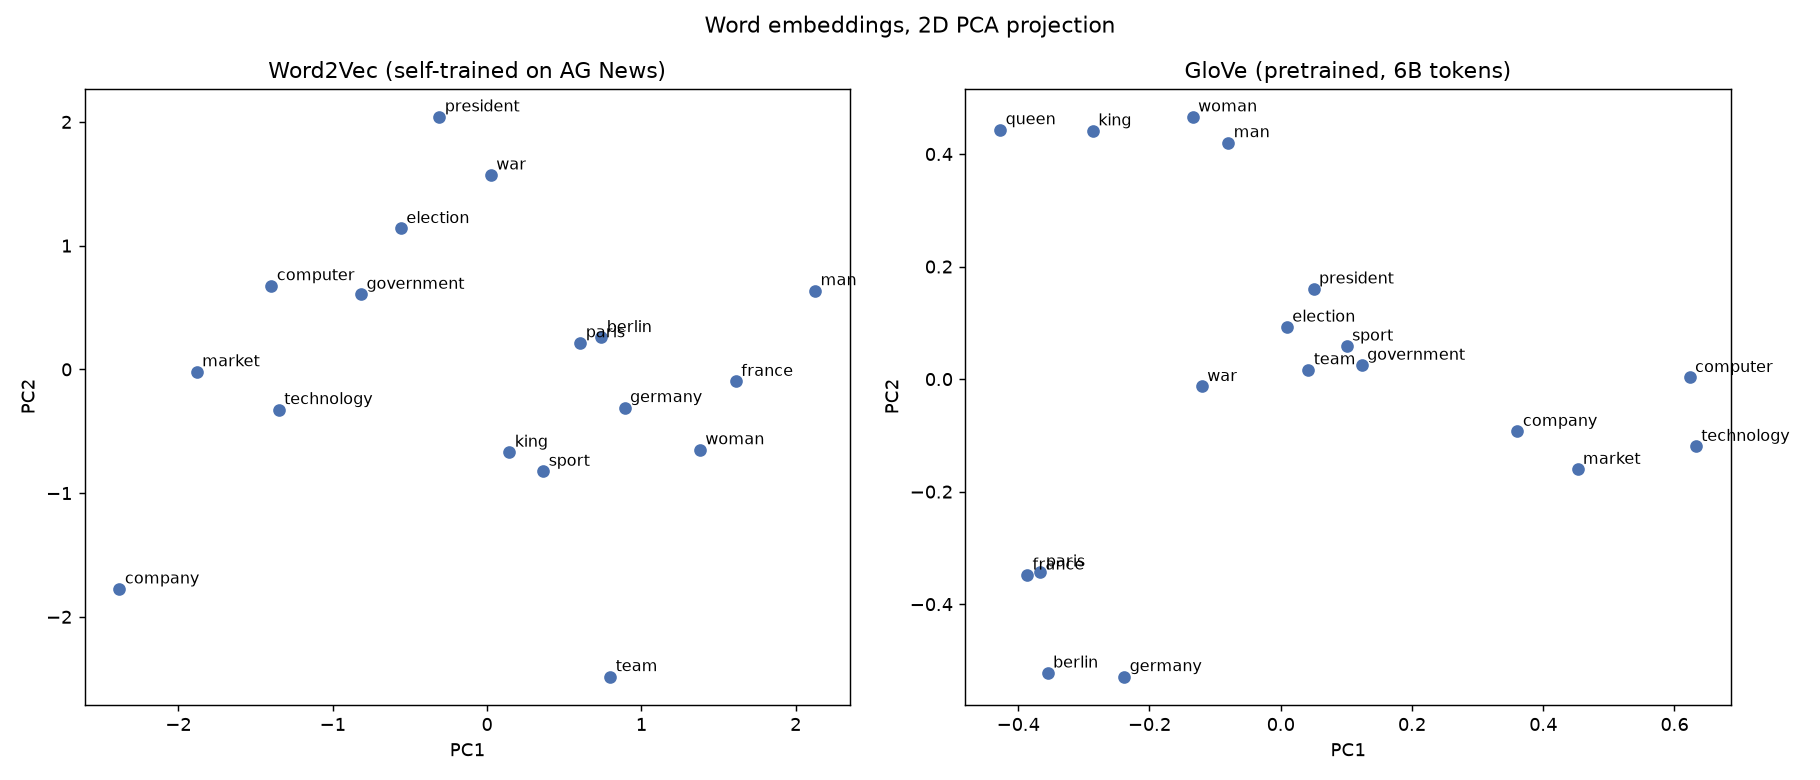
\includegraphics[width=0.95\textwidth]{figures/part_b_embeddings_pca.png}
    \caption{2D PCA projection: Word2Vec (self-trained) vs.\ GloVe (pretrained).}
\end{figure}

The visualization confirms this directly: GloVe's king/queen/man/woman and
paris/france/berlin/germany clusters are tight and well-separated; Word2Vec's corresponding
points are visibly noisier and less well-organized.

% ----------------------------------------------------------------
\section*{Part C: Applied Hugging Face Transformers Analysis}

\textbf{C1 -- tokenizer contrast.} DistilBERT's WordPiece tokenizer produces 13 tokens
(including \texttt{[CLS]}/\texttt{[SEP]}) for a 10-word sample sentence; Part A's toy BPE
(6-sentence training corpus vs.\ billions of words) produces 24 tokens on the identical
sentence, decomposing most words into short character fragments it never learned as merged
units. Same algorithm family (subword merge-based), vastly different training scale.

\textbf{C2 -- static embeddings vs.\ Word2Vec/GloVe.}

\begin{table}[H]
\centering
\begin{tabular}{lrrr}
\toprule
\textbf{Pair} & \textbf{DistilBERT (static)} & \textbf{Word2Vec} & \textbf{GloVe} \\
\midrule
king-queen & 0.657 & n/a$^*$ & 0.751 \\
king-car & 0.250 & 0.303 & 0.283 \\
man-woman & 0.650 & 0.462 & 0.832 \\
company-team & 0.415 & 0.152 & 0.461 \\
\bottomrule
\end{tabular}
\caption{$^*$``queen'' fell below Word2Vec's min\_count=5 frequency threshold in the small AG News subset.}
\end{table}

Different vector spaces/dimensionalities mean only the \emph{pattern} is comparable, not raw
values -- all three models agree king-queen and man-woman are markedly more similar than
king-car, a consistent qualitative signal across independently-trained embedding spaces.

\textbf{C3 -- contextual embeddings, polysemy demo.} The word ``bank'' extracted from
DistilBERT's final hidden layer across three sentences:

\begin{table}[H]
\centering
\begin{tabular}{lr}
\toprule
\textbf{Sentence pair} & \textbf{Cosine similarity} \\
\midrule
financial\_1 vs.\ financial\_2 (same sense) & \textbf{0.851} \\
financial\_1 vs.\ geographic (different sense) & 0.727 \\
geographic vs.\ financial\_2 (different sense) & 0.623 \\
\bottomrule
\end{tabular}
\end{table}

\begin{figure}[H]
    \centering
    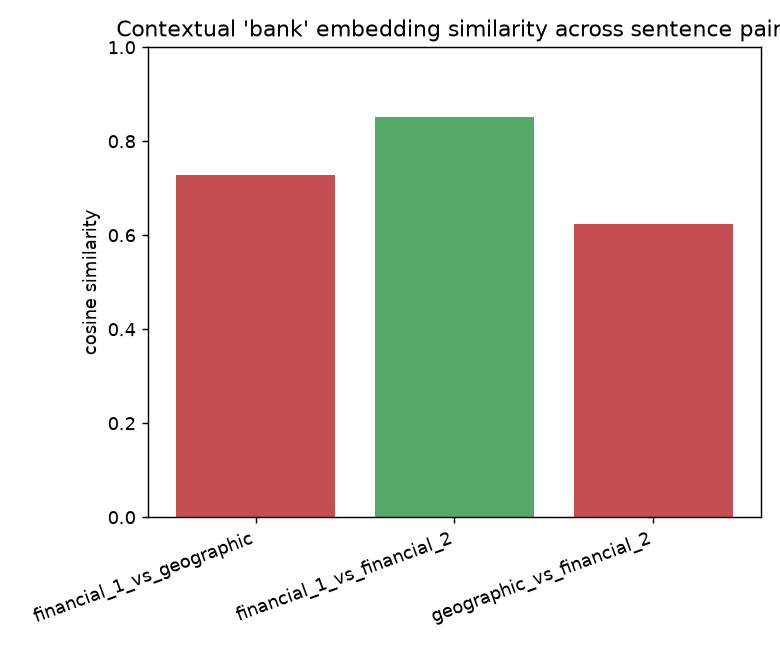
\includegraphics[width=0.6\textwidth]{figures/part_c_contextual_similarity.png}
    \caption{Contextual ``bank'' embedding similarity across sentence pairs.}
\end{figure}

Same-sense similarity (0.851) exceeds both different-sense pairs -- a measurable,
quantitative confirmation that contextual embeddings shift representation by word sense,
which a fixed Word2Vec/GloVe vector (Part B) structurally cannot do: one vector per word,
identical regardless of sentence.

\textbf{C4 -- OOV handling contrast.} WordPiece decomposes any unseen word into known
subword/character pieces -- there is no true OOV event at the tokenizer level, so the
embedding lookup always has a valid row to retrieve. Classical Word2Vec/GloVe have a
\emph{closed} vocabulary fixed at training time: a word absent from (or below min\_count in)
the training corpus has \textbf{no vector at all}, not a degraded approximation -- exactly
what happened to ``queen'' in Part C2's table above.

\textbf{C5 -- pipeline connection to Task 26.} The tokenizer converts text to token ids (no
learned parameters); the embedding layer maps ids to dense vectors via a learned lookup table
-- the \emph{first} learned computation in the pipeline, and exactly the $X$ matrix Task 26's
$Q{=}XW^Q, K{=}XW^K, V{=}XW^V$ projections are computed from. Positional encoding (Task 26
Part B2) is added directly to these same vectors, since self-attention has no inherent notion
of order. Every subsequent attention layer builds progressively more contextualized
representations on top of this initial embedding -- exactly what Part C3 observed directly:
the same input embedding for ``bank'' becomes sense-differentiated only \emph{after} passing
through attention layers, not at the embedding-lookup stage itself.

% ----------------------------------------------------------------
\section*{Part D: Analysis \& Documentation}

\textbf{D1 -- pipeline summary.} Tokenization (A) bounds vocabulary while preserving
meaningful OOV representation; sparse-vs-dense (B1) motivates embeddings amenable to
similarity arithmetic; Word2Vec (B2/B3) and GloVe (B4) are two paradigms for learning those
embeddings from corpus statistics, contrasted empirically in B5/B6; Hugging Face
tokenizer/embedding extraction (C) demonstrates the same conceptual pipeline at production
scale, composed with self-attention (Task 26) to become contextual rather than static --
directly bridging this task's classical-NLP foundations to Task 26's applied Transformer
analysis.

\textbf{D2 -- quantitative findings.} See B5/B6 and C2/C3's tables above: Word2Vec wins on
topical nearest-neighbors despite a tiny corpus but fails analogies; GloVe succeeds at both
given a $\sim$25,000x larger corpus; DistilBERT's static embeddings agree qualitatively with
both on relative word-pair similarity; DistilBERT's contextual embeddings measurably
separate word senses (0.851 same-sense vs.\ 0.727/0.623 different-sense), which static
embeddings cannot do by construction.

\textbf{D3 -- two implementation challenges.} (1) Early BPE testing risked merges spanning
word boundaries without the \texttt{</w>} end-of-word marker -- resolved by appending it to
every word before pair-counting, then manually verifying the merge log (\texttt{"low"+</w>},
\texttt{"new"+er}) contained only genuine within-word merges. (2) \texttt{gensim} failed to
build from source under this machine's default Python 3.14 (a \texttt{PyLongObject}/
\texttt{ob\_digit} Cython-internals error from extensions compiled against older CPython
APIs) -- diagnosed by reading the actual compiler error rather than assuming a
requirements-version mismatch, resolved by creating this task's virtual environment with
\texttt{python3.11} instead, under which gensim installs from a prebuilt wheel.

\textbf{D4 -- reflection.} Static embeddings' limitations are demonstrated concretely, not
just asserted: polysemy (C3's measured 0.851 vs.\ 0.727/0.623 similarity gap), fixed
vocabulary (C2's ``queen'' OOV event for Word2Vec), and general context-insensitivity. A
lightweight static-embedding approach remains preferable for \textbf{resource-constrained or
latency-critical deployment}: a Word2Vec/GloVe lookup is a single $O(1)$ array index, versus
a Transformer's $O(n^2d)$ self-attention (Task 26 Part B5) repeated across every layer just
to produce one contextual embedding. For applications where polysemy resolution isn't
essential -- a keyword-based document router, coarse topic-similarity search over short
queries, or an edge device with no practical way to run even a distilled Transformer -- a
static embedding table costs orders of magnitude less memory/compute for comparable value,
and remains more directly interpretable: a fixed per-word vector can be inspected and
clustered in isolation (Part B7's visualization) in a way a context-dependent vector, a
different point in space for every sentence, cannot be.

\end{document}
